\section{Results}

The VGG16 based flower classifier is trained on 50 epochs (about 45 minutes on GPU instance). According to Fig. \ref{VGG16_50e_Acc} and \ref{VGG16_50e_Loss}, the model achieve the best validation loss at epoch 33 with 0.2122. The validation accuracy stagnate at 90\% after the 10th epoch.

\begin{center}
	\centering
	\begin{minipage}{0.5\textwidth}
		\centering
		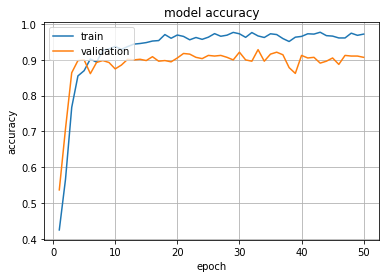
\includegraphics[width=0.9\textwidth]{./sections/04_results/output_33_0.png}
		\captionof{figure}{VGG16 - 50 epochs Accuracy}
		\label{VGG16_50e_Acc}
	\end{minipage}\hfill
	\begin{minipage}{0.5\textwidth}
		\centering
		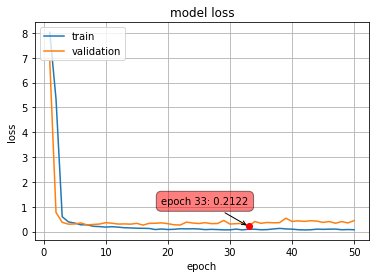
\includegraphics[width=0.9\textwidth]{./sections/04_results/output_33_1.png} 
		\captionof{figure}{VGG16 - 50 epochs Loss}
		\label{VGG16_50e_Loss}
	\end{minipage}
\end{center}

\subsection{Model Accuracy}

The model accuracy is compute by loading the best loss weights, scaling the test set and evaluating the model with its \texttt{evaluate} method on the scaled test dataset:
\\
The VGG16 based flower classifier achieve an accuracy of \textbf{89.30\%} on the testing set.

%\captionof{program}{best weights loading and evaluation of the model accuracy}
%\begin{python}
%base_model_name = 'VGG16'
%best_weights_h5 = 'saved_models/weights.best.flowers_recognition.{}.hdf5'.format(base_model_name)
%
%# load best loss weights
%model.load_weights(best_weights_h5)	
%
%# scale test dataset
%xtest_scaled = x_test.astype('float32')/255
%
%# evaluate model accuracy
%score = model.evaluate(xtest_scaled , y_test, verbose=1)
%
%# display accuracy in stdout
%print('\nTest accuracy: {:.2f}%'.format(score[1] * 100))
%\end{python}

\subsection{Justification}

The predictions are evaluated for each sample of the test dataset:

%\captionof{program}{test pictures prediction}
%\begin{python}
%import numpy as np
%
%predictions = np.array([np.argmax(model.predict(np.expand_dims(x, axis=0))) \
%	for x in tqdm(xtest_scaled)])
%\end{python}

The confusion matrix displayed in Fig. \ref{fig:output402} confirms the good performance of the model.

\begin{itemize}
	\item 80.7 \% of the test \textit{daisies} are correctly classified. The type of flower is mostly confused by the model by \textit{dandelions}.
	\item 92.6 \% of the test \textit{dandelions} are correctly classified. This type of flower is mostly confused by the model with \textit{sunflowers}. This remarquable score demonstrate that the model is able to identify the \textit{dandelions} both in yellows flower state and white "blow-balls" (see discussion in Chapter  \fullref{subsec:Data_exploration_and_visualization}). 
	\item 85.0 \% of the test \textit{roses} are correctly classified. This type of flower is mostly confused by the model with \textit{tulips}.
	\item 94.8 \% of the test \textit{sunflowers} are correctly classified. This the most accurately predicted type of flower. 
	\item 91.5 \% of the test \textit{tulips} are correctly classified. This type of flower is mostly confused by the model with \textit{roses}.
\end{itemize}

\begin{center}
	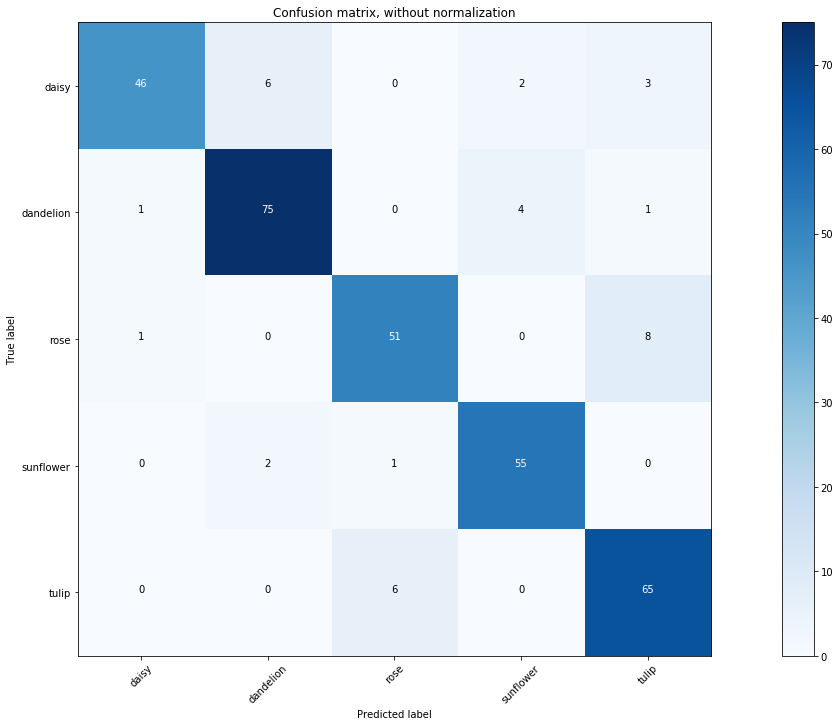
\includegraphics[scale=.4]{sections/04_results/output_40_2}
	\captionof{figure}{test pictures predictions - confusion matrix}
	\label{fig:output402}
\end{center}

The expectation to reach at least 80.0\% accuracy formulated in Chapter \fullref{subsec:benchmark} is met. Because the test pictures taken to evaluate the accuracy have never been seen by the model before, this good result let us suggest that the model is able to well generalize. The test samples displayed on Fig. \ref{fig:output420} demonstrate that the model is able to correctly identify:

\begin{itemize}
	\item single flowers on the picture
	\item multiple (two to several dozen) flowers on the same picture
	\item flowers taken from different angles
	\item same flower type in different life states (i.e. yellow flower and "blowball" dandelion)
\end{itemize}





